% !TeX root = ../main.tex
% Add the above to each chapter to make compiling the PDF easier in some editors.

\chapter{Evaluation}\label{chapter:evaluation}
\begin{figure*}[htbp]
    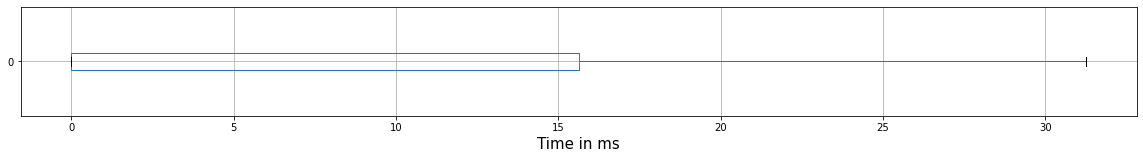
\includegraphics[width=\textwidth,height=\textheight,keepaspectratio]{logos/PurePythonLatencies.png}
     \caption{Time between two frames in a python client}
    \label{fig:PythonFPS}
\end{figure*}
The latencies shown in the following graphs are measured with a video from the
Youtube-8M dataset \parencite{abuelhaija2016}. The video is 4 minutes and 22.94 seconds long and consists of 6,569 frames. Moreover, an average of five replays is used. For consistency, the gaze is fixed in the middle of the frame at the coordinates \((960,512)\). Nevertheless, no loss in latency is measurable when the gaze changes. The overall latency is calculated by sending a time-step from the server to the client. This timestamp is evaluated after the image is shown on the display. This method leads to an overall latency measurement including every step. The image upscaling is at first a linear interpolation. Additionally, the client starts before the server to guarantee an optimal stream initialisation from the beginning.

\begin{table}
\centering
\begin{tabular}{ c | c }
\hline
 Codec & Latency \\ [0.5ex] 
\hline\hline
 WebRTC & ca. 500ms \\ 
 H.265  & ca. 250ms \\  
 H.264  &   >1s     \\  
 VP9    & ca. 1s    \\
 AV1    &   >10s    \\  
\end{tabular}
\caption{Comparison of the latency of the different codecs}
\label{table:comparisoncodecs}
\end{table}


\begin{figure*}[htbp]
    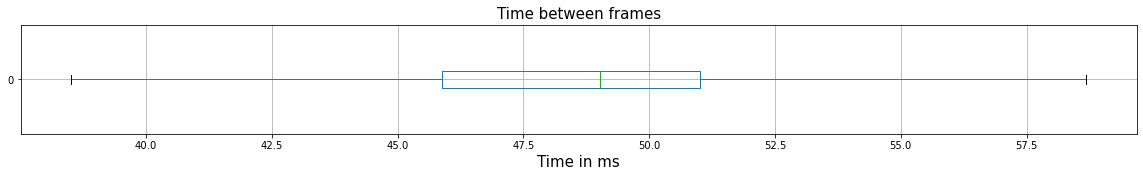
\includegraphics[width=\textwidth,height=\textheight,keepaspectratio]{logos/Unity3DFPS.png}
    \caption{Time between two frames in the Unity3D}
    \label{fig:UnityFPS}
\end{figure*}

\par
After selecting the possible codecs, the different codecs are compared against each other in terms of latency. Stating in \autoref{table:comparisoncodecs}, WebRTC and H.265 achieve the lowest latency. It is to mention that the AV1 codec has currently no hardware encoding and decoding available and therefore is not usable in this setup. Also, the H.264 codec specifies to buffer some frames in any case and cannot be disabled, resulting in this higher latency. As the H.265 is slightly faster with the parameters given in the former section, it was further evaluated. WebRTC could perform better, but due to a time constraint as the implementation differs completely, it was not further considered.
\par

\par
At first, it was proven with \autoref{fig:PythonFPS} that the server and the client deliver constant frames in a specific time limit with a Python client. As seen in \autoref{fig:PythonFPS}, the time between two frames is not more than 30ms, which results in a minimum of 33 FPS. The outliers reach up to 400ms, as the initialisation needs some time and thus the client cannot deliver continuous images during the first few seconds. This scenario is also visible in the image, as it is pixelated in the beginning but then stabilises. The corresponding Unity3D client needs 32–58ms as stated in \autoref{fig:UnityFPS} between each frame and therefore works correctly.

\begin{figure}[htbp]
    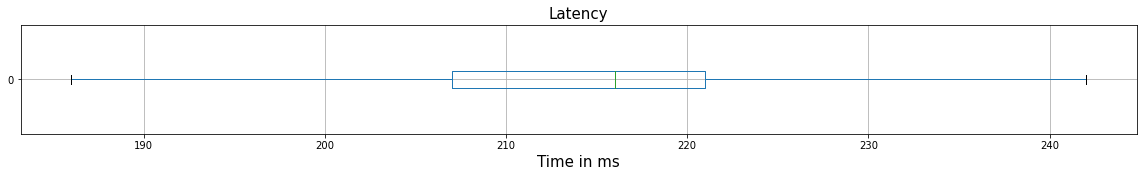
\includegraphics[width=\textwidth,height=\textheight,keepaspectratio]{logos/Unity3dWithoutOutliers.png}
    \caption{Latency of Unity3D}
    \label{fig:UnityLatenyVRWithoutOutliers}
\end{figure}

\begin{figure}[htbp]
    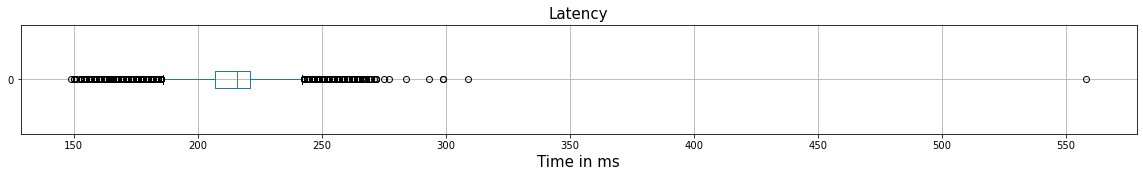
\includegraphics[width=\textwidth,height=\textheight,keepaspectratio]{logos/Unity3dWithOutliers.png}
    \caption{Complete latency of Unity3D with outliers}
    \label{fig:UnityLatenyVRWithOutliers}
\end{figure}

\par 
To measure the latency, different modes were compared. At first, it was determined if there is any impact on the increased hardware demand when the \gls{vr} is enabled or disabled. Furthermore, the differences between the available bandwidths were determined.

\begin{figure}[htbp]
    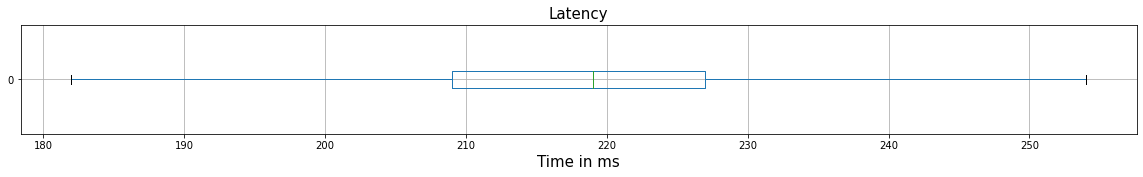
\includegraphics[width=\textwidth,height=\textheight,keepaspectratio]{logos/Unity3dVRWithoutOutliers.png}
    \caption{Latency including enabled\gls{vr}}
    \label{fig:VRLatency}
\end{figure}

\par
When \gls{vr} is disabled and the available bandwidth is not limited, the resulting latency ranges from 172–230ms, whereas the average latency is 219ms as visible in the boxplot of \autoref{fig:UnityLatenyVRWithoutOutliers}. Having a span of 57ms indicates that the transmission is stable, and it also emphasises that there is a continuous frame. Furthermore, there is minimal difference in the latency between when the \gls{vr} is enabled and disabled, which means that the additionally needed hardware power does not impact the streaming as stated in \autoref{fig:VRLatency}.

\begin{figure}[htbp]
    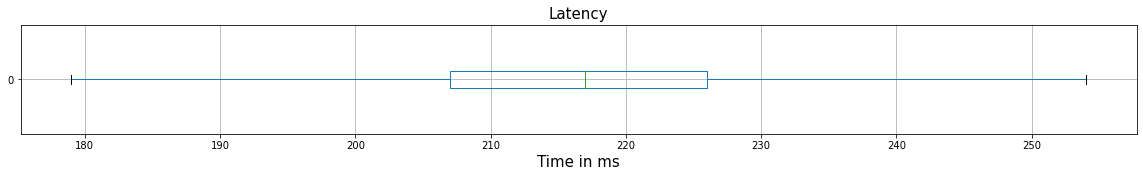
\includegraphics[width=\textwidth,height=\textheight,keepaspectratio]{logos/LowBandwidth.png}
    \caption{Latency with 640 kilobits per second bandwidth}
    \label{fig:lowbandwidthlatency}
\end{figure}

\par
The latency stays the same for a broad span of the available bandwidth. When the bandwidth drops to 640 kilobits per second, the latency does not change as the \autoref{fig:lowbandwidthlatency} indicates. When the rate drops below this line, not every benchmark ran successfully as FFmpeg desynchronised and therefore no stable transmission could be determined.
\par 
The test of the superresolution requires to have a standardised training process. Therefore, each model is trained with 20,000 epochs with the DIVK dataset. The batch size is set to 1 as not more images fit into the VRAM with a crop size of 128. The batch size defines the number of training examples utilized in one training period. In this case, the training example contains two images, a low-resoltion image and the corresponding high-resolution image. As the full training needs at least a day to train, not every model is trained thoroughly. The models differ in the amount of the residual blocks, which repeats 4, 8, 12 or 16 times often. This method allows comparing multiple models for latency. For association, the models are compared against the linear and the bicubic interpolation in terms of latency and quality.

\begin{figure}[htbp]
    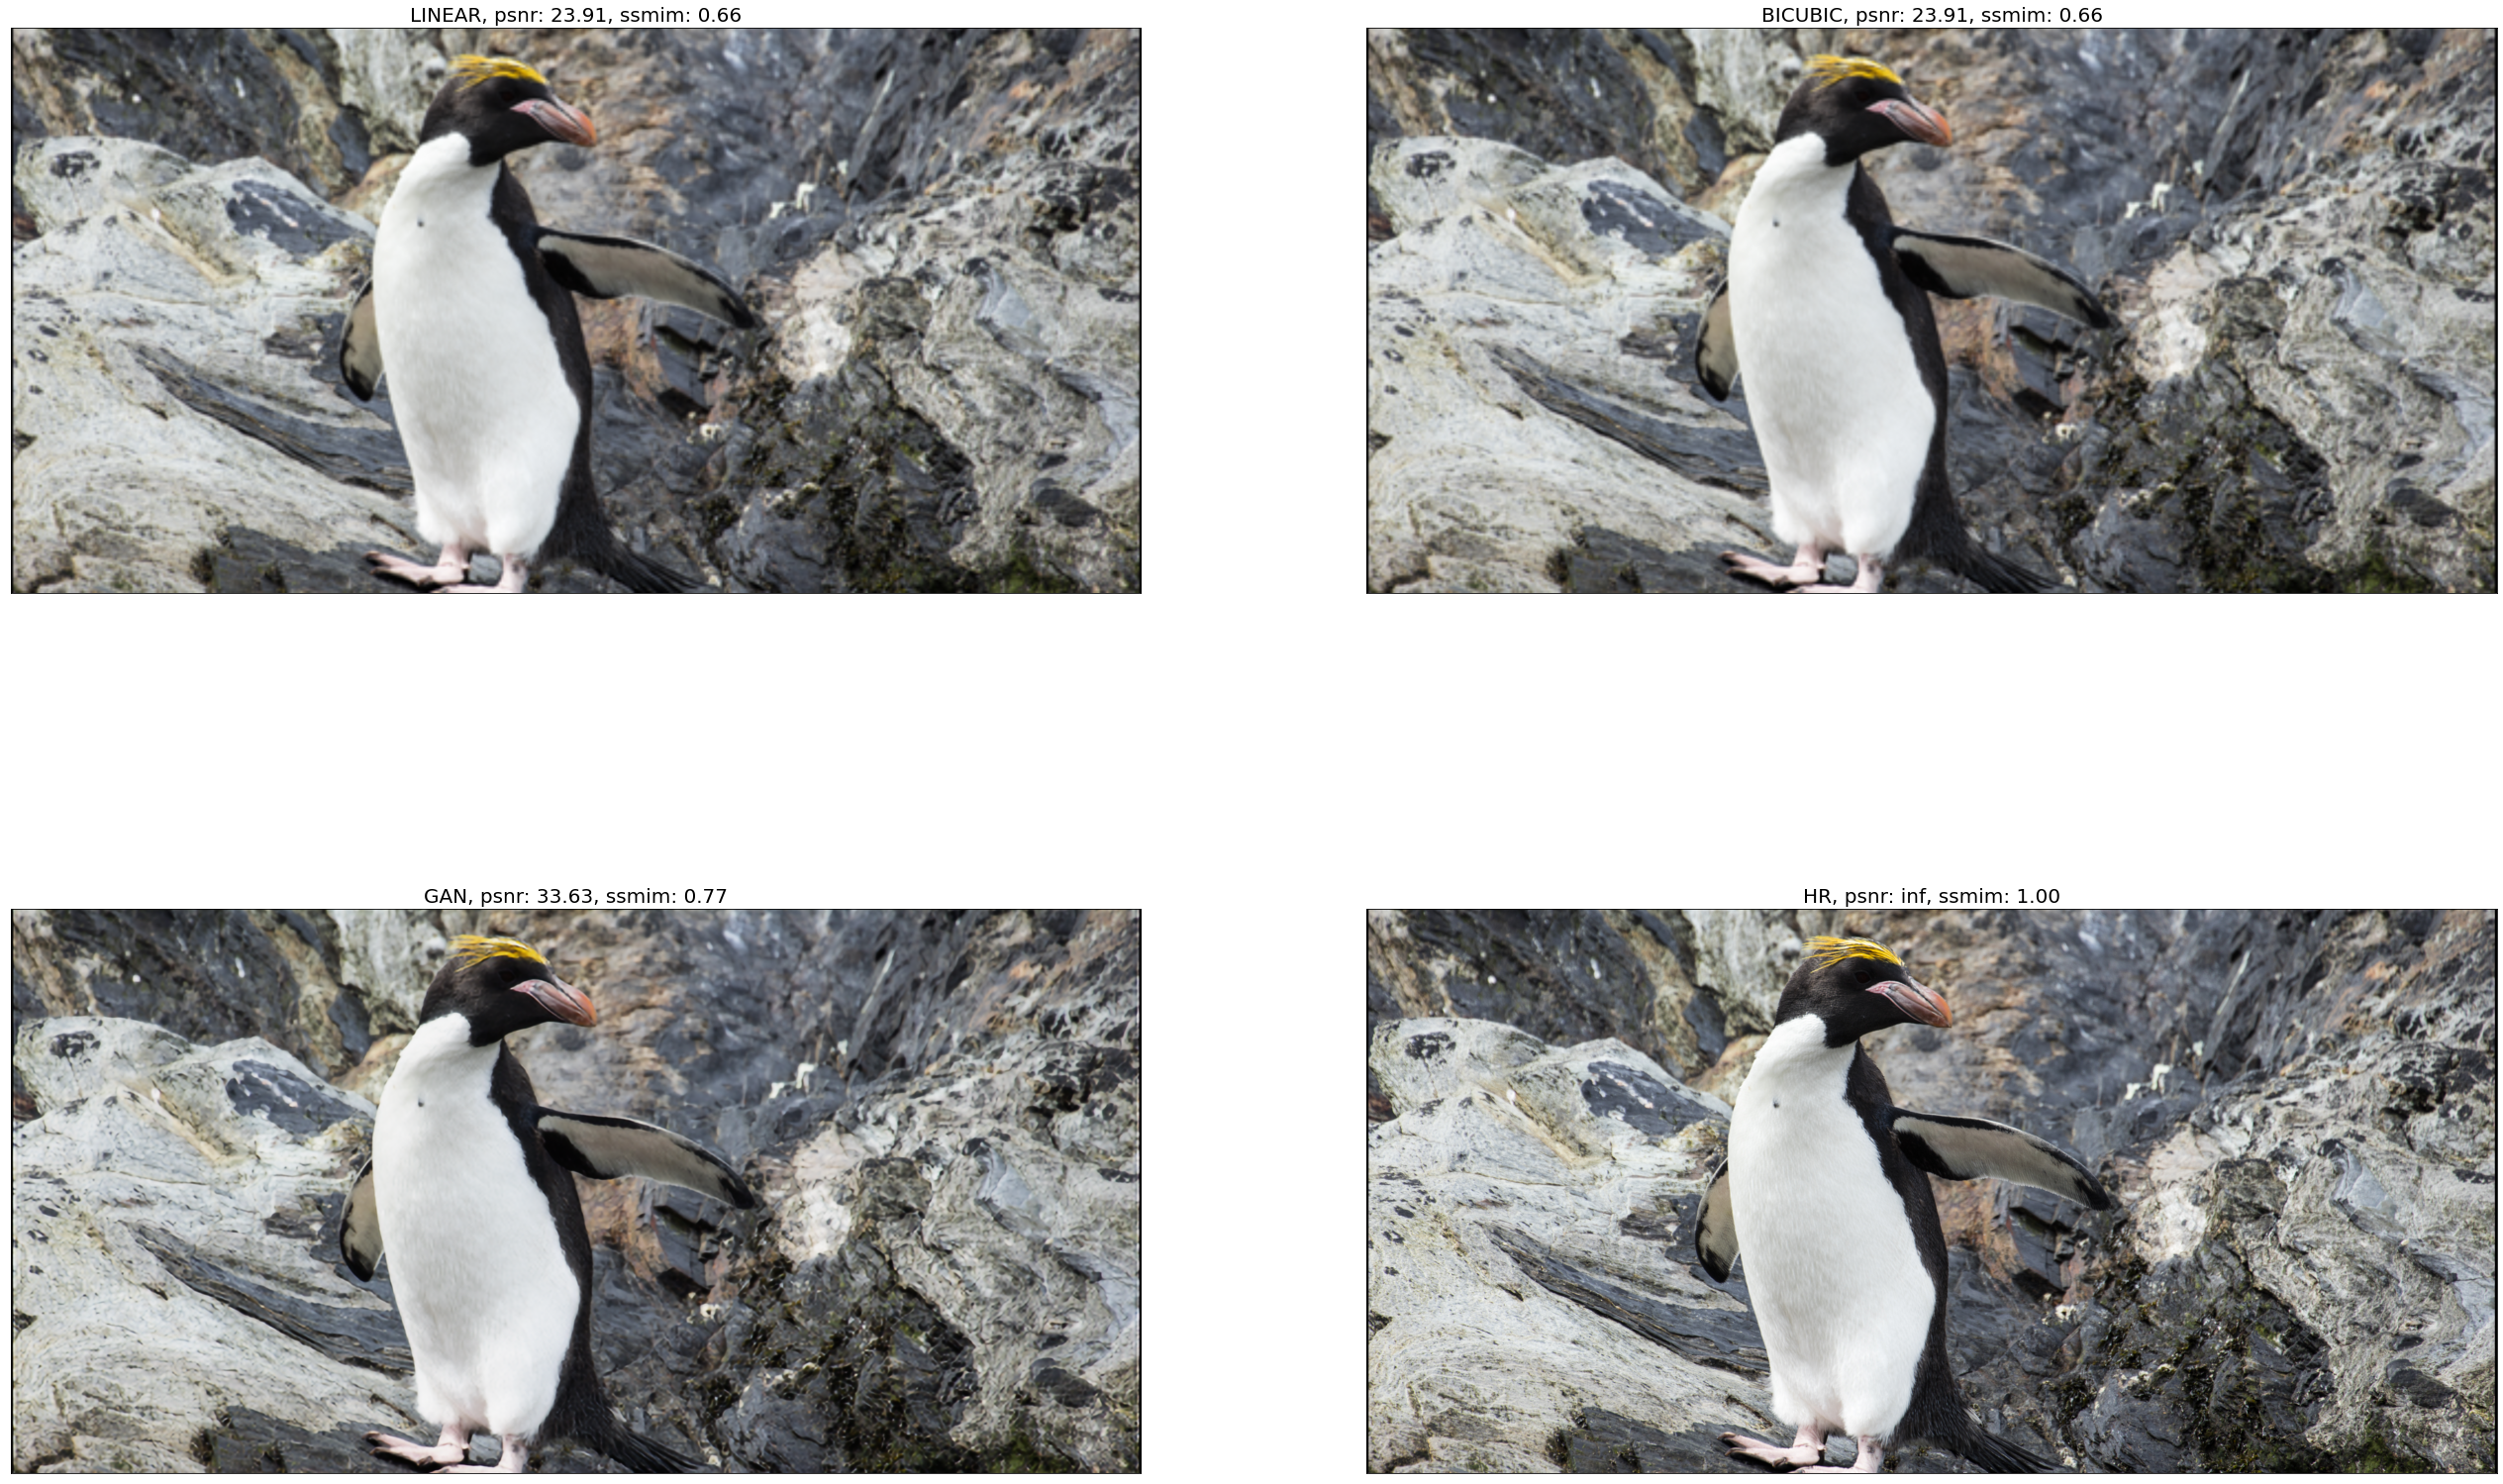
\includegraphics[width=\textwidth,height=\textheight,keepaspectratio]{logos/GANPerformance.png}
    \caption{Performance of a \gls{gan} model in comparison to linear and bicubic interpolation. The image is taken from the DIVK dataset \parencite{Agustsson2017}}
    \label{fig:ganperformance}
\end{figure}

\par
The presented superresolution, which replaces the linear or bicubic upsampling, performs well. It performs the upscaling better than other standard methods. As seen in \autoref{fig:ganperformance}, the peak signal-to-noise ratio (PSNR) value signals the ratio between the maximum possible power of an image and the power of corrupting noise affecting the quality. Moreover, the \gls{ssim} also indicates a better quality, which leads to the result that in terms of superresolution, the neural network beats the standard methods. The speed between the different models differs slightly for a few milliseconds, as stated in \autoref{fig:modellatency}.
\par
Alternatively, the neural network is much slower than the interpolation upsample methods, but it improves the image better. The linear upsampling needs approximately 1ms, which is the fastest method. It delivers acceptable quality in comparison to the neural network, which needs approximately 20ms and creates a better image quality. However, this only relates to the pure network. Furthermore, some other operations add 40ms to the latency, such as a conversation from the float32 type back to the uint8 type, independent of the network.


\begin{figure}[htbp]
    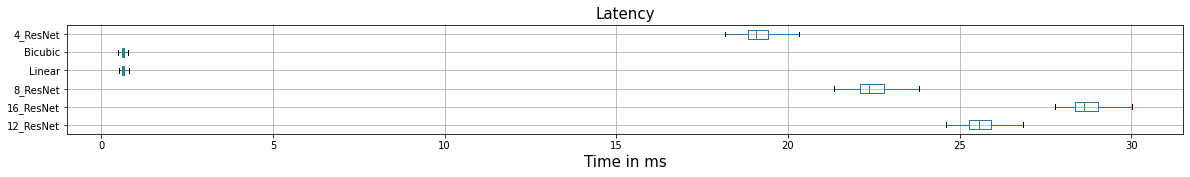
\includegraphics[width=\textwidth,height=\textheight,keepaspectratio]{logos/latencyUpscaling.png}
    \caption{: Latency of the \gls{gan} models in comparison to linear and bicubic interpolation.}
    \label{fig:modellatency}
\end{figure}
